% v2-acmtog-sample.tex, dated March 7 2012
% This is a sample file for ACM Transactions on Graphics
%
% Compilation using 'acmtog.cls' - version 1.2 (March 2012), Aptara Inc.
% (c) 2010 Association for Computing Machinery (ACM)
%
% Questions/Suggestions/Feedback should be addressed to => "acmtexsupport@aptaracorp.com".
% Users can also go through the FAQs available on the journal's submission webpage.
%
% Steps to compile: latex, bibtex, latex latex
%
% For tracking purposes => this is v1.2 - March 2012
\documentclass{acmtog} % V1.2
\usepackage{amsmath}
\usepackage{bm}
%\acmVolume{VV}
%\acmNumber{N}
%\acmYear{YYYY}
%\acmMonth{Month}
%\acmArticleNum{XXX}
%\acmdoi{10.1145/XXXXXXX.YYYYYYY}
\acmVolume{28}
\acmNumber{4}
\acmYear{2019}
\acmMonth{January}
\acmArticleNum{106}
\acmdoi{10.1145/1559755.1559763}

\begin{document}

\markboth{Pruning Algorithm}{Reconstructive net pruning using ADMM}

\title{Reconstruction net pruning using ADMM} % title

\author{Hao Zhang {\upshape and} Zixuan Chen
\affil{Shanghai Jiao Tong University}
% NOTE! Affiliations placed here should be for the institution where the
%       BULK of the research was done. If the author has gone to a new
%       institution, before publication, the (above) affiliation should NOT be changed.
%       The authors 'current' address may be given in the "Author's addresses:" block (below).
%       So for example, Mr. Fogarty, the bulk of the research was done at UIUC, and he is
%       currently affiliated with NASA.
}


\maketitle


\section{Introduction}
In this project, we apply several neural network compression algorithms to the inverting image network to test the robustness of these algorithms. Specifically, we use the reconstruct net from the paper \emph{ Inverting Visual Representations with Convolutional Networks} and compress this network. We extract features of these images from the fourth and fifth hidden layer from the AlexNet and use the Cifar-10 dataset as a replacement of the ImageNet. We then apply the ADMM algorithm from the paper \emph{A Systematic DNN Weight Pruning Framework using Alternating Direction Method of Multipliers} to compress and retrain the pretrained network. At last, we compare the performance(including the value of loss function and the quality of the inverted images) of the nets before and after prunning.

\section{Background and related works}
\label{sec:background}
\subsection{AlexNet}

AlexNet is firstly proposed by A.Krizhevsky, I.Sutskever and G.E.Hinton in 2012. And this model got the champion in the ImageNet competition in 2012. This model successfully used some tricks such as ReLU, Dropout and LRN. AlexNet is considered one of the nost influential papers published in computer vision, having spurred many more papers published employing CNNs and GPUs to accelerate deep learning.
\subsection{Inverting image}
Feature representations are always hard to analyze, and we can learn the representations by inverting an image from a reconstruct network. There are many approaches to invert an image. According to the work of A.Dosovitskiy and T.Brox, we can extract features from the hidden layer of a CNN and inverting an image with several convolutional layers and up-convolutional layers. In A.Dosovitskiy's work, they used AlexNet and get a good result to invevrt images.
\subsection{introduction to ADMM algorithm}

ADMM was first introduced in the 1970s, and theoretical results in the following decades have been collected in \cite{Background}. It is a powerful method for solving regularized convex optimization problems, especially for problems in applied statistics and machine learning. 

For some problems which are difficult to solve directly, we can use variable splitting first, and then employ ADMM to decompose the problem into two subproblems that can be solved separately and efficiently. For example, the op-timization problem.
\begin{equation}
  minimize_x\mbox{ }f(x) + g(x)
\end{equation}

assumes that f(·) is differentiable and g(·) is non-differentiable but has exploitable structure properties. To make it suitable for the application of ADMM, we use variable splitting to rewrite the problem as
	
\begin{eqnarray*}
  minimize_x\mbox{ }f(x) + g(x)\\
  \mbox{subject to }x = z
\end{eqnarray*}
more details of ADMM algorithm will be illustrated in section~(\ref{sec:proposed_methods})
\section{Motivation}

Nowadays, deep neural networks play an important role in many fileds, such as image classification, natural language processing, image semantic segmentation and so on. But it's getting more difficult to train a deep networks since the parameters become more and more. Although there are several effective methods to decrease the number of parameters, such as using convolutional layer, using smaller convolutional kernel, sometimes it's still necessary to design compress algorithm to simplify the network to get a better training speed.\\

There are already some methods to decrease the complexity of the network. However, as far as we know, these algorithms are mainly applied on the classifiers and use the accuracy as an index to judge whether this algorithm will affect the performance. And most of these algorithms will adjust the loss function, which will lead to a slightly increasement of original loss. Since the accuracy only focus on the largest or the five largest channels, we think it can not totally reflect the affaction of the compression algorithm. So we decide use another model and choose a compress algorithm to test its robustness.\\

We choose the reconstruct net and ADMM algorithm because this net can make the result more visible and clear to human.
\section{Problem Formulation}
\label{sec:problem_formulation}

\begin{figure}[h]
  \centerline{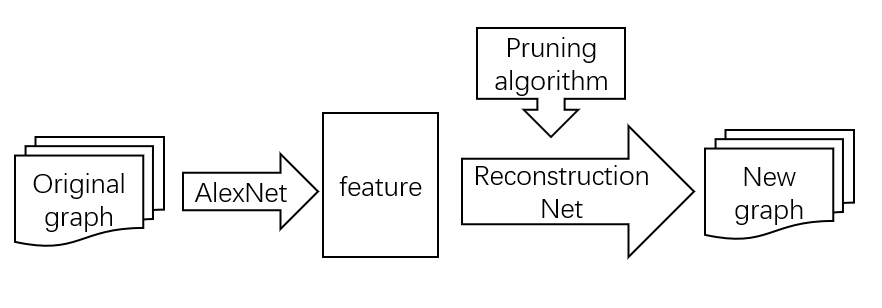
\includegraphics[width=7cm]{graph/pf_4.png}}
  \caption{problem formulation}
\end{figure}
Our problem is to reconstruct graph from features generated from AlexNet and then generate proper algorithm to prune the reconstruction net.
The origin AlexNet is trained with ImageNet, ,which is too large for us to train, \subsection{Inverting image}
The origin AlexNet is trained with ImageNet, ,which is too large for us to train, so we firstly adjusted and trained our own AlexNet with a smaller dataset Cifar-10. Then we extract images' features from the fourth and fifth layer respectively and build two reconstruct nets to invert images. We used the parameters from A.Dosovitskiy's work. The construct of these two models are shown in the Table1.\\
\begin{table}
\centering 
\begin{tabular}{c|c|c}
\hline
&reconstruct v1&reconstruct v2\\
\hline
from layer&4th&5th\\
\hline
feature size&4*4*128&8*8*96\\
\hline
conv num&3&3\\
\hline
conv K/S&3/1&3/1\\
\hline
convt num&3&2\\
\hline
convt K/S&5/2&5/2\\
\hline
\end{tabular}
\caption{}
\end{table}
In the Table1, K represents the kernel size and S represents the strides of the kernel. When these two models are trained, we can apply our algorithms to compress them.

\subsection{Problem formulation of weight pruning}
Assume we want to prune a fully connected DNN layers, and suppose we have input \textbf{x}, the output \textbf{h} of the fc layer will be
$$h = \sigma(Wx + b)$$
where \textbf{h} and \textbf{b} have t columns. The nonlinear activation function $\sigma()$ acts entrywise on its arguments, and is typically chosen to be the ReLU function. the output of the i-th layer will be 
$$h_i =\sigma(W_ix + b_i) $$
Suppose we input a batch of images, the output of the DNN will be
$$y = W_Nh_{N-1} + b_N$$
in this case s is a $k\times t$ matrix. The loss function of this DNN is illustrated as\\
% $$f({W_1,...,W_N}, {b_1, ..., b_N}) = -\frac{1}{t}\sum_{j = 1}^t\frac{e^{s_{y_jj}}}{\sum_{i = 1}^ke^{s_{ij}}$$
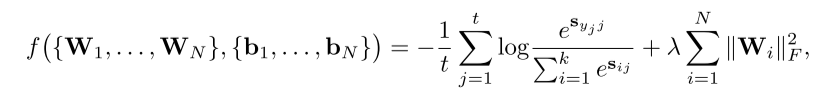
\includegraphics[scale = 0.4]{graph/pf_5.png}
where $||\cdot||_F^2$ denote the Frobenius norm, the first term is the cross entropy loss, the second term is the l2 loss, and the second term is the l2 regularization term. The training of DNN is a process of minimizing the loss by updating weight W and bias b
\begin{align*}
  W_i &= W_i - \alpha\frac{\partial f({W_i}{b_i})}{\partial W_i}\\
  b_i &= b_i - \alpha\frac{\partial f({W_i}{b_i})}{\partial b_i}\\
\end{align*}
for i = 1, ..., N and $\alpha$ is the learning rate.\\
Our objective is to prune the weights of the DNN, and therefore we minimize the loss function subject to constraints on the cardinality of weights in each layer.More specifically, our training process solves\\
\begin{figure}[h]
  \centering{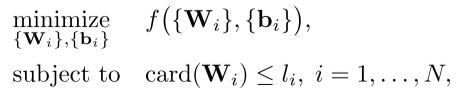
\includegraphics[scale = 0.5]{graph/pf_6.png}}
\end{figure}\\
where card return the number of nonzero element of the given matrix and $l_i$ is the desired number of each layer.
\section{Proposed Methods-ADMM}
\label{sec:proposed_methods}
In the above section we discussed the problem formulation of weight pruning as
\begin{figure}[h]
  \centering{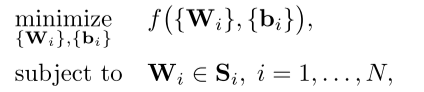
\includegraphics[scale = 0.5]{graph/pm_1.png}}
\end{figure}\\
where $S_i = {W_i | card(W_i) \leq l_i}, i = 1,...,N$. It is clear that $S_1, ..., S_N$ are nonconvex sets, and it is general difficult to solve optimization problem with nonconvex constraints. the problem can be equivalently rewrittern in a form without constraints, which is \\
\begin{equation}\label{equ:problem}
\mathop {minimize}_{\{W_i\},\{b_i\}} f(\{W_i\}\{b_i\}) + \sum_{i=1}^Ng_i(W_i)
\end{equation}
where $g_i(·)$ is the indicator function of $S_i$, i.e.,\\
\begin{equation*}
  g_i(W_i) = \begin{cases}
    0\mbox{ if }card(W_i)\leq l_i\\
    +\infty\mbox{ otherwise}
  \end{cases}
\end{equation*}
The first term of problem ~\ref{equ:problem} is the loss function of a DNN, while the second term is non-differentiable. This problem cannot be solved analytically or by stochastic gradient descent. We begin by equivalently rewriting the above problem in ADMM form as
\begin{equation*}\label{equ:problem_rewrite}
  \mathop {minimize}_{\{W_i\},\{b_i\}} f(\{W_i\}\{b_i\}) + \sum_{i=1}^Ng_i(Z_i)\\
  \mbox{subject to }W_i = Z_i, i = 1, ..., N
\end{equation*}
The augmented Lagrangian of the above optimization problem is given by
\begin{figure}[h]
  \centering{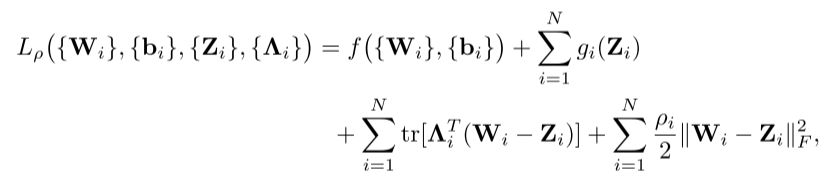
\includegraphics[scale = 0.4]{graph/pm_2.png}}
\end{figure}\\
If we define the scaled dual variable $U_i = (1/\rho_i)\Lambda_i$, the augmented lagrangian can be equivalently expressed as 
\begin{figure}[h]
  \centering{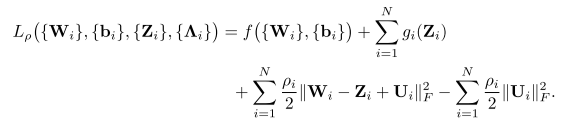
\includegraphics[scale = 0.6]{graph/pm_3.png}}
\end{figure}\\
The ADMM Algorithm proceeds by repeating, for k = 0,1,..., the following steps:
\begin{align}
  \{W_i^{k+1}\}\{b_i^{k+1}\} &:= \mathop{argmin}_{\{W_i\},\{b_i\}}L_{\rho}(\{W_i\},\{b_i\},\{Z_i^k\},\{U_i^k\})\\
  {Z_i^{k+1}} &:= \mathop{argmin}_{\{Z_i\}}L_{\rho}(\{W_i^{k+1}\},\{b_i^{k+1}\},\{Z_i\},\{U_i^k\})\\
  U_i^{k+1} &:= U_i^k + W_i^{k+1} - Z_i^{k+1}
\end{align}
until both of the following conditions are satisfied.\\
\begin{equation}
  \lVert W_i^{k+1}, b_i^{k+1}\rVert_F^2 \leq \epsilon_i, \lVert Z_i^{k+1} - Z_i^k\rVert_F^2 \leq \epsilon_i
\end{equation}
problem (3) can be formulated as 
\begin{equation*}\label{equ:problem_3}
  \mathop {minimize}_{\{W_i\},\{b_i\}} f(\{W_i\}\{b_i\}) + \sum_{i=1}^N\frac{\rho_i}{2}\lVert W_i - Z_i^k + U_i^k \rVert_F^2\\
\end{equation*}\\
ans problem (4) can be formulated as 
\begin{equation*}\label{equ:problem_3}
  \mathop {minimize}_{\{Z_i\}}\sum_{i=1}^Ng_i(Z_i) + \sum_{i=1}^N\frac{\rho_i}{2}\lVert W_i^{k+1} - Z_i + U_i^k \rVert_F^2\\
\end{equation*}\\
\section{Experiments}
\subsection{Partly compress}
\label{sec:experiments}
We decided to finish our experiment step by step, so we decide to firstly compress the convolution layers only and check whether the algorithm can compress the network effectively. Then we will compress all the layers to test its robustness.\\
We have chose 3 layers of reconstruction net, that is, the first 3 convolutional layers of reconstruction net to apply our ADMM algorithm. we compare the original graph, the recontructed graph by the original reconstruction net as well as the reconstructed graph by the pruned Reconstruction net. We calculate the nonzero weight values and the weight distribution of each Reconstruction net. And the result is as follows.
\begin{figure}[!h]
  \label{fig:res0}
  \centering
  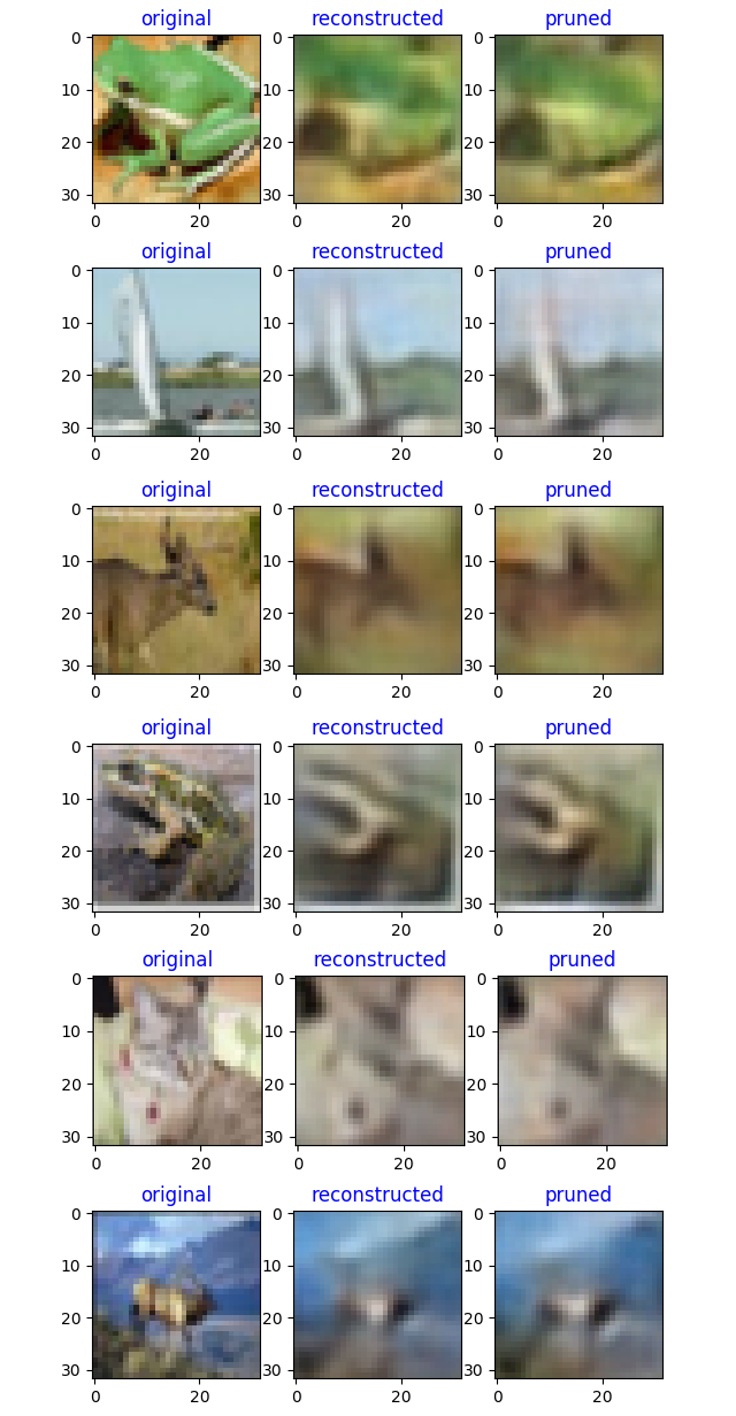
\includegraphics[scale = 0.65]{graph/exp_1.png}
  \caption{the original graph, the recontructed graph by the original reconstruction net as well as the reconstructed graph by the partly pruned Reconstruction net}
\end{figure}
From figure2 we can see that the recontructed graphs generated from the original reconstruction net are quite different from the original graph due to the higher fuzzy degree. What is amazing is there is small difference between he recontructed graph by the original reconstruction net as well as the reconstructed graph by the pruned Reconstruction net.
\begin{figure}[!h]
  \label{fig:res1}
  \centering
  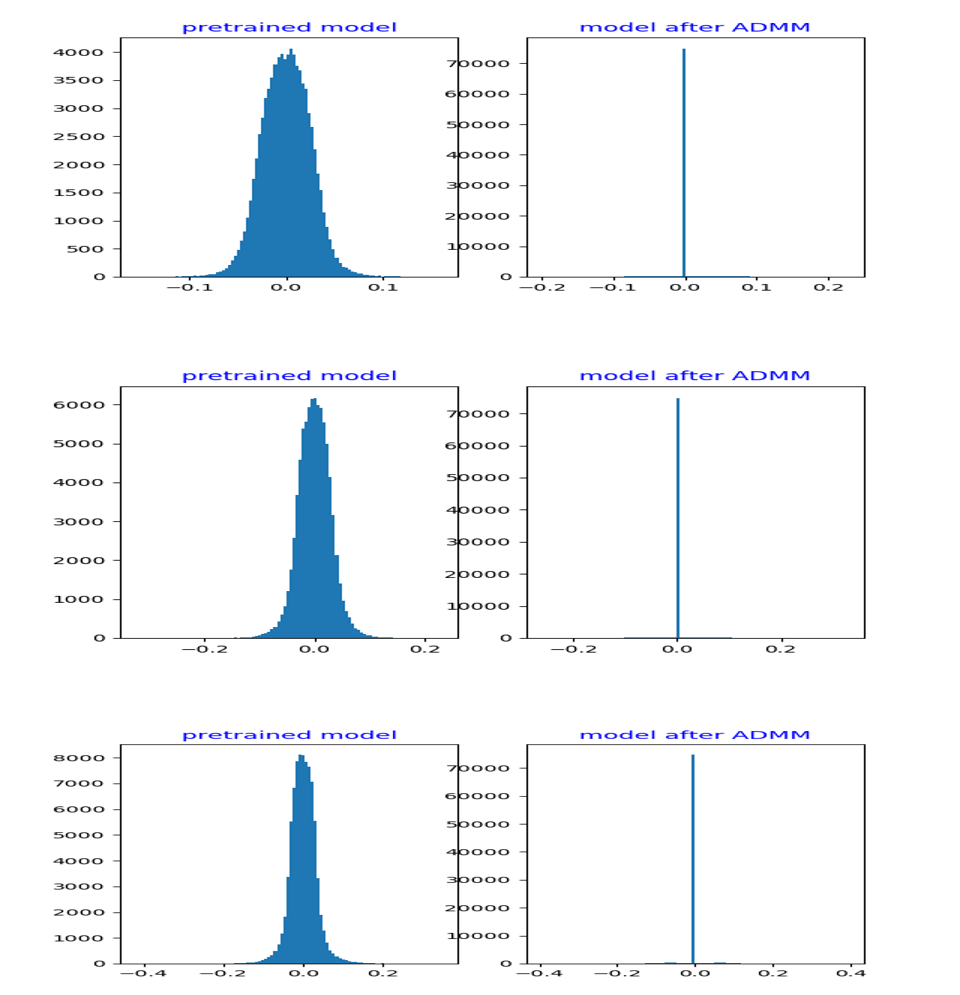
\includegraphics[scale = 0.65]{graph/exp_2.png}
  \caption{the weight distribution of each Reconstruction net, the first row is the conv1 layer, the second row is the conv2 layer, the third row is the conv3 layer (partly compress)}
\end{figure}
We can see that before pruning, each layer have different distribution. After pruning process, most of the weight values  of each convolutional layer have become zero. From the figure3 and figure4 we can see that almost 90\% of the weight value have been pruned.
\begin{figure}[!h]
  \label{fig:res2}
  \centering
  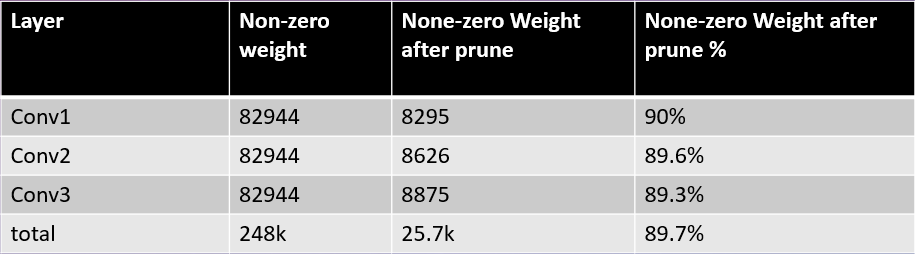
\includegraphics[scale = 0.3]{graph/exp_3.png}
  \caption{the weight distribution of each Reconstruction net, the first row is the conv1 layer, the second row is the conv2 layer, the third row is the conv3 layer (partly compress)}
\end{figure}
From the above experiments, we can see that the ADMM algorithm is very practical for image reconstruction. However, there is slightly little challenge in balancing the  prune rate to secure the degree of accuracy.
\subsection{Complete Compress}
Since it's useful to apply this algorithm to the reconstruct net, we moved on and compress all the layers. This step is more challenge for the algorithms because the up-convolutional layers are quite important for the inverting images. We test this algorithm with the features from the fourth hidden layer and the fifth hidden layer of the AlexNet. And we need one more up-convolutional layer to prune when inverting images from the fifth layer. In this step, we fix the compress rate at 0.9 and retrain enough epoches to get a precise number of nonzero weight values.And the inverting results of the two model are as follows.\\
\begin{figure}[h]
  \label{fig:res3}
  \centering
  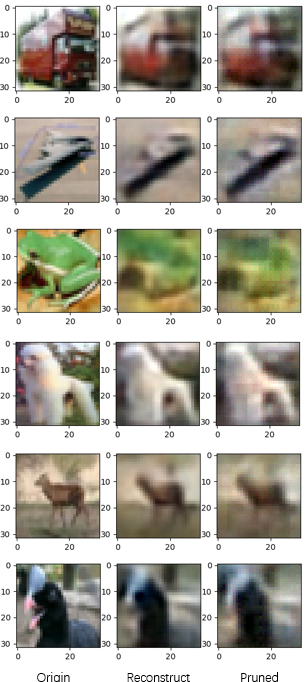
\includegraphics[scale = 0.65]{graph/exp4_result.png}
  \caption{the original graph, the recontructed graph by the original reconstruction net as well as the reconstructed graph by the pruned Reconstruction net, features from the fourth layer}
\end{figure}
\begin{figure}[h]
  \label{fig:res0}
  \centering
  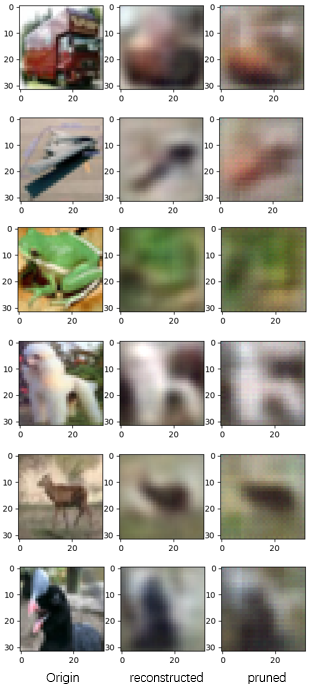
\includegraphics[scale = 0.65]{graph/exp5_result.png}
  \caption{the original graph, the recontructed graph by the original reconstruction net as well as the reconstructed graph by the pruned Reconstruction net, feaetures from the fifth layer}
\end{figure}
According to the figure5 and figure6, we can see that figure5 has a better performance than figure6, which is easy to understand because inverting an image from a deeper layer is more difficult. However, when we observe the result of the pruned net, we can easily find that the performance of pruned nets are clearly worse than the origin reconstruct net. Comparing with the result of the part compress, we know that this is because we prune the up-convolutional layers. What's worse, the difference between the two nets of figure6 is larger than the two nets of figure5 and the pruned net in figure6 sometime even make mistakes about the color.
\section{Conclusion and Future Work}
In this paper, we apply ADMM algorithm in image reconstruction net. We formulated the process of Inverting an image and pruning a DNN layers. We then introduced the detailed mathematical derivation of ADMM algorithm. We use AlexNet to extract features of the original image and reconstruct the image using the reconstruction net. Then we apply ADMM algorithm to prune the reconstruction net.\\
In the experiment, we find that when we apply this algorithm to all the layers in the net, the affact caused by the algorithms becomes more visible due to the representation of inverting images.\\
In the future, we plan to compress reconstruction network from layer 5 of Alexnet. In the mean time, we plan to try to combine ADMM algorithm with quantization.
\label{sec:conclusion}
%
% Start of "Sample References" section
\newpage
\appendix
\section{Reference}
\label{sec:cmds}
\bibliographystyle{plainnat}
\begin{thebibliography}{1}
  \bibitem{Background} 1. Boyd, S., Parikh, N., Chu, E., Peleato, B., Eckstein, J.: Distributed optimization and statistical learning via the alternating direction method of multipliers.
  Foundations and Trends  in Machine Learning 3(1) (2011) 1–122
  \bibitem{algor}2. Zhang T , Ye S , Zhang K , et al. A Systematic DNN Weight Pruning Framework using Alternating Direction Method of Multipliers[J]. 2018.
  \bibitem{algor}3. Dosovitskiy A, Brox T. Inverting Visual Representations with Convolutional Networks[C]// IEEE Conference on Computer Vision \& Pattern Recognition. 2016.
  \bibitem{algor}4. Krizhevsky A, Sutskever I, Hinton G E. ImageNet classification with deep convolutional neural networks[C]// International Conference on Neural Information Processing Systems. 2012.
\end{thebibliography}

\end{document}
% End of v2-acmtog-sample.tex (March 2012) - Gerry Murray, ACM
